\documentclass[nogrid]{MBE_article}%

\usepackage{url}

\jshort{mst}

\volname{}

\jvolume{0}

\jvol{}

\jissue{0}

\pubyear{2016}

\mstype{Letter}

\artid{012}

\access{Advance Access publication November 2, 2016}


\begin{document}

\title[BuddySuite]{BuddySuite: Command-line toolkits for manipulating sequences, alignments, and phylogenetic trees}


\author[Bond et al.]{Stephen R. \surname{Bond}, Karl E.
Keat, Sofia N. Barreira, and Anreas D. Baxevanis$^{\ast}$}

\address{Computational and Statistical Genomics Branch, Division of Intramural Research, National Human Genome Research Institute, National Institutes of Health, 50 South Drive, Bethesda, MD, USA, 20892}


\history{Received 12 November 2016}

\coresp{E-mail: andy@mail.nih.gov}


\editor{???}

\abstract{The ability to manipulate sequence, alignment, and phylogenetic tree files has become an increasingly important skill in the life sciences, whether it be to generate summary information or to prepare data for further downstream analysis. The command-line is an extremely powerful environment for interacting with these resources, especially as files become even moderately large, but there has been little focus on developing or maintaining general-purpose toolkits in recent years.
BuddySuite is a collection of four independent yet interrelated command-line programs that facilitate each step in the workflow of sequence discovery, curation, alignment, and phylogenetic reconstruction. Most common sequence, alignment, and tree file formats are automatically detected and parsed, and over 100 tools have been implemented for manipulating this data. The project has been engineered to easily accommodate the addition of new tools, it is written in the popular programming language Python, and is hosted on the Python Package Index and GitHub to maximize accessibility. Documentation for each BuddySuite tool, including usage examples, is available at http://tiny.cc/buddysuite\_wiki.
\newline
All software is open source and freely available at http://research.nhgri.nih.gov/software/BuddySuite}

\keyword{software, command line, sequence, alignment, phylogenetic tree, python, toolkits}


\maketitle


\section{{Introduction}\label{sec:Intro}}
Manipulation of biological sequence data is now a routine task within the life sciences, not just by bioinformaticians, but also by `bench biologists' who are becoming increasingly savvy in applying computational methods to their own work. While there are excellent graphical platforms for organizing, visualizing, and manipulating these forms of data, it is often advantageous to interact with text files directly from the command line, especially when the size of datasets become even moderately large. Most common tasks can be accomplished with existing open source software, but it is usually necessary to bring together many different standalone tools to build a particular workflow. Such tools may be dependent on pre-defined file format specifications, have non-trivial installation requirements, and/or be difficult to extend or modify. While each of these issues is surmountable, particularly if one can write custom programs in any of the popular scripting languages (e.g., bash, Perl, R, or Python), they do impose an entry barrier to those without a basic background in computer science. Furthermore, finding available tools can be difficult, as specialized programs are not generally well advertised or highly ranked by search engines. To address these issues we have developed BuddySuite, a unified set of command-line data manipulation tools that are easy to install, intuitively organized, and implemented in the popular programming language Python. This software is particularly geared for individuals with a basic working knowledge of the UNIX shell environment who routinely interact with sequence, alignment, or phylogenetic tree files.

\section{Implementation}
BuddySuite is a set of Python 3 libraries and command-line applications developed for use on all major operating systems (Windows 7+, Mac OSX, and Linux) and leverages the sequence and phylogenetic tree processing capabilities of Biopython \cite{Cock:2009hj}, Environment of Tree Exploration 3 (ETE3) \cite{HuertaCepas:2016hw}, and Dendropy \cite{Sukumaran:2010id}. The software is free and open-source, versioned on Github \cite{github} and the Python Package Index \cite{pypi} (PyPI), and unit tested at a code coverage of over 95\%.

\subsection{Installation}
Stable release versions of BuddySuite can be installed directly from PyPI using the popular package manager `pip', and development versions from GitHub are also easily installed using the provided setup script. While optional, users are also encouraged to run the BuddySuite configuration script after installation:

\smallskip
{\small
\begin{verbatim}
 $: buddysuite -setup
\end{verbatim}
}
\smallskip
Doing so will create directories for caching data on the user's system and will register an email address for the tools that interact with public databases (to prevent possible IP blocking). To simplify installation, dependencies have been limited to packages available through PyPI, although there are a number of optional third-party programs that can be accessed through BuddySuite; these include BLAST \cite{Camacho2009} for comparing sequences, multiple sequence alignment packages like MAFFT \cite{Katoh:2013hm}, and phylogenetic inference packages like RAxML \cite{Stamatakis:2006de}. As these programs are not necessary for the general operation of the BuddySuite modules, installation is the user's responsibility. The third-party tools that BuddySuite wraps are itemized in table \ref{table:software}.

\begin{table}[!t]
\tableparts{\caption{List of optional third party software that BuddySuite programs can interact with.\label{table:software}}}
      {\tabcolsep=5pt\begin{tabular}{@{\extracolsep{\fill}}lll@{}}
      \toprule
	   						& Program								& Reference
      \\\colrule
      SeqBuddy			& BLAST 								& \cite{Camacho2009}
      \\\colrule
      AlignBuddy		& Clustal$\Omega$					& \cite{Sievers:2011fn} \\
        					& ClustalW2 							& \cite{Larkin:2007hz} \\
							& MAFFT 								& \cite{Katoh:2013hm} \\
							& MUSCLE 								& \cite{Edgar:2004bo} \\
							& PAGAN 								& \cite{Loytynoja:2012fy} \\
        					& PRANK 								& \cite{Loytynoja:2005cb}		
      \\\colrule
      PhyloBuddy		& FastTree							& \cite{Price:2010eg} \\
        					& RAxML 								& \cite{Stamatakis:2006de} \\
        					& PhyML 								& \cite{Guindon:2010gf}
      \\\botrule
      \end{tabular}}
{\tablenote{BuddySuite performs all necessary format conversion to call any of these tools and, where appropriate, returns the result in the same format as the input. This is particularly useful when creating multiple sequence alignments from annotated sequences in GenBank or EMBL format.}}
\end{table}

\subsubsection{Command-line user interface}
The four core command-line programs distributed with BuddySuite are SeqBuddy, AlignBuddy, PhyloBuddy, and DatabaseBuddy. The first three accept sequence, alignment, or phylogenetic tree data as input, respectively, using flags to switch among the tools available in each program. All output is printed directly to the terminal window by default and each module adheres to the UNIX convention of accepting piped data, allowing individual tools to be `daisy-chained' into more complex workflows. DatabaseBuddy, on the other hand, is intended to run primarily as a `live shell', allowing the user to interactively search and download sequence data stored in the NCBI, UniProt, and Ensembl public databases. At the time of writing, 104 individual tools have been implemented across the BuddySuite programs.


\subsubsection{Documentation}
Basic help is available for each BuddySuite module from the command line by passing in the `-h' or `-{}-help' flag. Doing so will generate a list of all tools along with brief usage instructions. Extended documentation has also been prepared in markdown for every tool, complete with an explanation for any arguments and fully worked usage examples. These resources are maintained as a separate repository on GitHub and are rendered as a public wiki (http://tiny.cc/buddysuite\_wiki).

\subsubsection{Application programing interface (API)}
Each module has a core `Buddy' class that automatically handles a variety of input types (e.g., plain text, file paths or handles, or a list of Biopython objects), performs all necessary file format processing, and exposes methods for managing and writing the sequence or tree records. All of the API functions in each library accept these `Buddy' objects as input and generally return them as output, thus providing a standardizing interface that facilitates interoperability among functions. Once installed, the BuddySuite libraries can be imported into third-party scripts using the standard Python syntax.

\subsubsection{Error reporting and usage statistics}
Looking forward, the modular nature of BuddySuite makes it particularly well suited for continued growth. New tools are easily added to each existing module and new modules may eventually extend the suite to new data types. Instead of relying on active community input to identify bugs and drive future development, we have implemented an optional passive data collection system to monitor usage and to report crashes. This data is transmitted to an FTP server after all personally identifiable information has been stripped away. This also allows us to immediately inform users of available bug fixes; a crash traceback can be combined with a module's version number to create a unique identification hash and, once identified, these hashes are stored in the Git repository along with their status (i.e., pending or resolved). If an update is available that will fix a particular issue, the user will be informed at the time of the crash.

\section{Results and Discussion}
\subsubsection{The unique features of BuddySuite}
The European Molecular Biology Open Software Suite (EMBOSS) and Biopieces are the most comprehensive general-purpose opensource bioinformatics toolkits currently available for the command line. While both are excellent software packages, the development of BuddySuite is justified by a number of key differences. In particular is our switch away from the `one program per function' paradigm that EMBOSS and Biopeices employ (each suite contains about 200 separate programs). BuddySuite groups all functions related to a particular data type together into specific modules and uses flags to differentiate among them; this reduces the potential for naming collisions on a user\rq{}s system PATH. BuddySuite is also the only general-purpose toolkit implemented entirely in pure Python. This is unlike EMBOSS, which must be compiled primarily from C, and Biopieces, which relies on Python, Perl, and Ruby. While there is a performance cost when running an interpreted language like Python,  it makes installation easier and it reduces the entry barrier for public contribution to the project. Python and R have now emerged as the main prototyping and scripting languages in the life sciences \cite{Ekmekci:2016co}, largely due to the growing number of researchers who are learning to program for the general purpose of data wrangling \cite{Hannay:2009hv}. This positions BuddySuite as a more approachable option for users who wish to implement custom functionality.

To keep the learning curve as shallow as possible, care has been taken to minimize the number of parameters each tool depends upon and to use duck typing to infer user intent. For example, the SeqBuddy `find\_restriction\_sites' function is one of the most flexible in the suite; it can accept three different argument types that control what enzymes are included in the search and how the output is formatted, yet all of these arguments are optional and can be passed to the tool in any order. This flexibility is in contrast to EMBOSS and BioPieces, which generally require extra flags to explicitly set all parameters. When the argument type (e.g., integer or string) unambiguously identifies how it should be used by the tool, we believe it is counter-productive to impose positional constraints or additional flags. Furthermore, file format detection is fully automated. Any number of sequence, alignment, or phylogenetic tree files can be passed into their respective BuddySuite program, in any combination of supported formats, and the records will be parsed seamlessly (see table \ref{table:formats} for a list of supported formats). This is particularly useful when using the BuddySuite modules to call third party alignment or phylogenetic inference programs, as any idiosyncratic format conversions are handled without further input from the user. For a general purpose tool like BuddySuite, where the user is intended to interact with their data dynamically on the command line, we believe that minimizing key-strokes is crucial.

\begin{table}[!t]
\tableparts{\caption{File format support for reading (R) and writing (W) provided by each BuddySuite module.\label{table:formats}}}
      {\tabcolsep=4pt\begin{tabular}{@{\extracolsep{\fill}}llll@{}}
        \toprule
        Format							& SeqBuddy  					& AlignBuddy   					& PhyloBuddy
        \\\colrule
        Clustal 						& R \& W\textsuperscript{\dag} 	& R \& W						& None \\ 
        EMBL\textsuperscript{\ddag} 	& R \& W						& R\textsuperscript{\dag}/ W	& None \\
        FASTA 							& R \& W						& R\textsuperscript{\dag}/ W	& None \\
        GenBank\textsuperscript{\ddag} 	& R \& W						& R\textsuperscript{\dag}/ W 	& None \\
        Nexus 							& R \& W\textsuperscript{\dag}	& R \& W						& R \& W \\ 
        Newick 							& None							& None							& R \& W \\ 
        NeXML							& None							& None							& R \& W \\
        PHYLIP (interleaved)			& R \& W\textsuperscript{\dag} 	& R \& W						& None \\
        PHYLIP (sequential)				& R \& W\textsuperscript{\dag} 	& R \& W						& None \\	
        SeqXML							& R \& W						& None							& None \\ 
        Stockholm						& R \& W\textsuperscript{\dag} 	& R \& W						& None \\ 
        Swissprot\textsuperscript{\ddag}& R only						& None							& None
        \\\botrule
      \end{tabular}}
{\tablenote{\textsuperscript{\dag}All sequences must be the same length \\
      		  \textsuperscript{\ddag}Supports rich sequence annotation}}
\end{table}

Perhaps the greatest advantage BuddySuite has over other tools is its handling of annotations. Rich flat-file formats like GenBank and EMBL support sequence feature annotation, but this information is generally discarded by the EMBOSS programs and the Biopieces suite is unable to write these formats. SeqBuddy and AlignBuddy are both aware of features in the sequence records they process and will update those annotations when sequences are modified. For example, if a group of DNA sequences are translated into protein sequences with SeqBuddy, the relative positions of each feature will be scaled by one third to account for the conversion of codons to amino acids. If those proteins are then passed to AlignBuddy to create a multiple sequence alignment, the features will be adjusted again to account for any gaps that are introduced. Unfortunately, support for the Generic Feature Format (GFF3) specification is not currently implemented in BioPython, so is also not available in BuddySuite at the time of writing. While GFF3 support is planned for a future release, users are currently encouraged to write annotated sequences to GenBank or EMBL; this includes alignments, as BuddySuite will respect gap characters in these formats.

\begin{figure*}[t]
\begin{center}
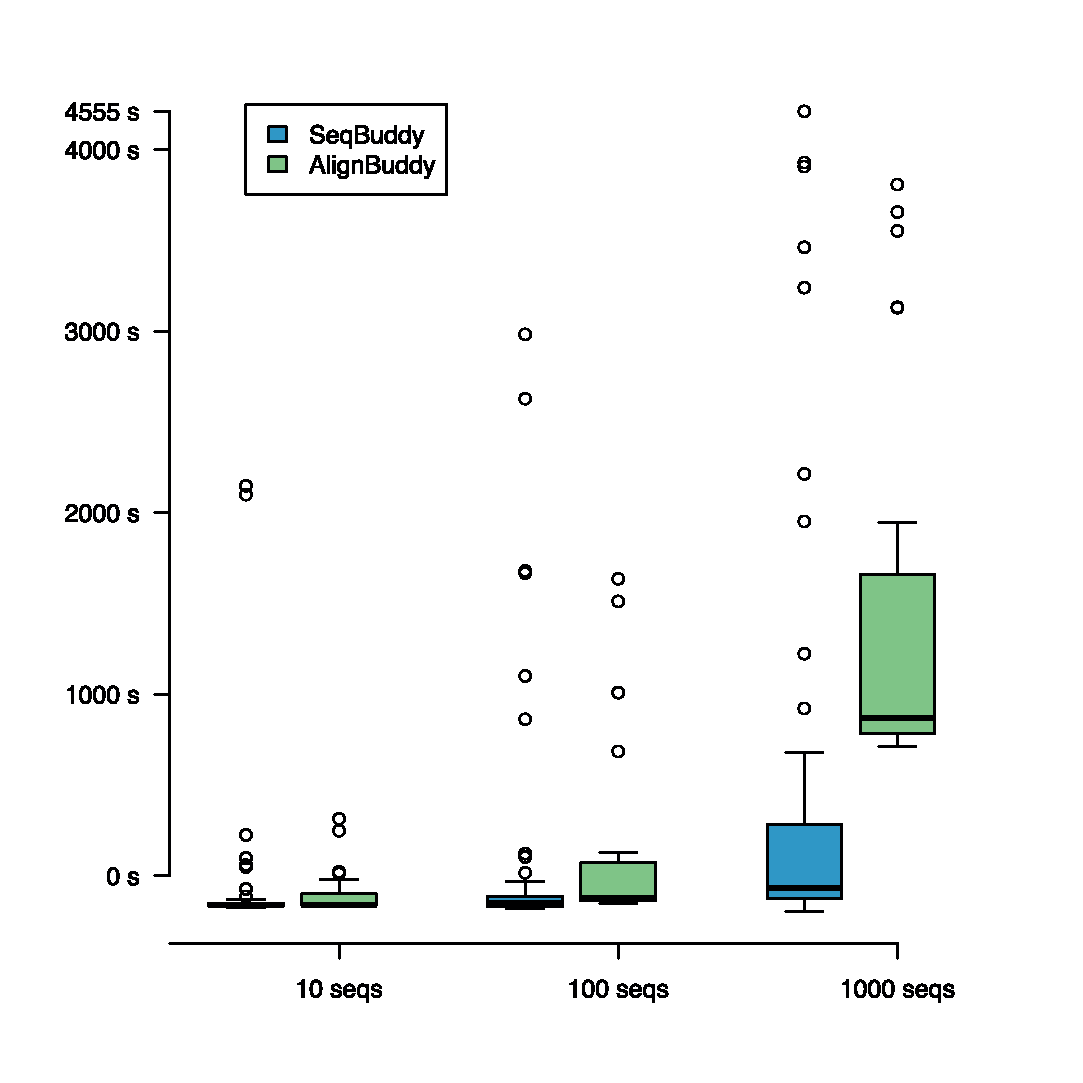
\includegraphics[height=0.4\textheight]{figures/timeit.eps}
\end{center}
\caption{Runtimes for each BuddySuite tool. All tools not dependent on third-party resources were executed in triplicate using sample datasets of 10, 100, and ~1000 records on [SOFIA'S HARDWARE]. Average runtimes are expressed in seconds and the y-axis is log-scale.}
\label{fig:timeit}
\end{figure*}

\subsubsection{Use-case examples}
BuddySuite modules are executed from the command line using the following generalized syntax:

\smallskip

{\small
\begin{verbatim}
 $: module file(s) <cmd> <args> <modifiers>
\end{verbatim}
}
\smallskip

Any number of files may be passed into the module but only a single command can be executed at a time. As a specific example, the following would accept two sequence files (in FASTA and GenBank formats) and delete any sequences larger than 300 residues (module names have been shortened in the following examples to sb, alb, and pb for SeqBuddy, AlignBuddy, and PhyloBuddy, respectively):

\smallskip

{\small
\begin{verbatim}
 $: sb seqs1.gb seqs2.fa --delete_large 300
\end{verbatim}
}
\smallskip

Whichever format is encountered last will be the format the final records will be output as (in this case, FASTA), although this behaviour may be overridden with the `-{}-output' modifier:

\smallskip

{\small
\begin{verbatim}
 $: sb seqs1.gb seqs2.fa --delete_large 300
    --output genbank
\end{verbatim}
}
\smallskip

Keeping with the spirit of inferring user intent, modifiers are used sparingly in the BuddySuite modules and only when their effects are intuitively applicable across all tools in the module (e.g., quiet execution or to modify files in-place).

The BuddySuite modules also accept input from standard output, allowing for the construction of more complex workflows using the pipe character. In the following example, SeqBuddy pulls out records with RefSeq identifiers (using a regular expression), AlignBuddy calls MAFFT to generate an alignment and shifts gaps to force a codon alignment, then PhyloBuddy calls RAxML to infer a phylogeny before rooting the tree at its midpoint.

\smallskip
{\small
\begin{verbatim}
 $: sb sequences.gb --pull_records "[XN]M\_" |
    alb --generate\_alignment mafft |
    alb --enforce\_triplets |
    pb --generate\_tree raxmlHPC-SSE3 |
    pb --root
\end{verbatim}
}

\smallskip
Third-party programs that use any of the supported file formats and utilize standard output and standard input from the command line can also be seamlessly included in these pipelines.

\subsubsection{Performance}
Performance is a key disadvantage when implementing bioinformatics software in an interpreted language, such as Python, compared to compiled languages like C or C++.
The primary trade-off an interpreted language over a complied language for BuddySuite, is performance. While careful use of Python's core data-types can dramatically improve the performance of the software, it will not compare to C.

Here are some graphs and tables showing how long each tool takes to run on different sized files. Include reference to BamTools and SamTools here, explaining why this is such a different project. See figure \ref{fig:timeit}.

\begin{table}[!t]
\tableparts{\caption{Runtimes for each BuddySuite tool.\label{table:timeit}}}
      {\tabcolsep=5pt\begin{tabular}{@{\extracolsep{\fill}}llcccc@{}}
      \toprule
	   				& Dataset Size	& 25\%		& 50\%		& 75\%		& max
      \\\colrule
      SeqBuddy		& 10				& 0.715	& 0.722	& 0.733	& 1.570 \\
      				& 100				& 0.711	& 0.728	& 0.776	& 9.049 \\
						& 1000			& 0.778	& 0.850	& 1.315	& 83.83
		\\\colrule
      AlignBuddy	& 10				& 0.724	& 0.728	& 0.749	& 1.876 \\
      				& 100				& 0.762	& 0.786	& 0.974	& 26.39 \\
						& 1000			& 4.811	& 5.680	& 14.22	& 2032.0
		\\\colrule
      PhyloBuddy	& 10				& 1.702	& 1.717	& 1.737	& 3.010 \\
      				& 100				& 1.747	& 1.757	& 1.770	& 3.549 \\
						& 1000			& 1.637	& 1.657	& 1.693	& 4.546
      \\\botrule
      \end{tabular}}
{\tablenote{All tools not dependent on third-party resources were executed in triplicate using sample datasets of 10, 100, and ~1000 records on [SOFIA'S HARDWARE]. Runtime percentiles are expressed in seconds.}}
\end{table}

\section{Conclusions}
BuddySuite has been designed from the ground up as an intuitive, extensible, and unified platform for routine command-line tasks performed on sequence, alignment, and phylogenetic tree files. This is the first time such a large suite of general-purpose bioinformatics utilities have been implemented purely in Python and packaged together under a flag-driven paradigm. Well-designed and actively supported open-source tools will be invaluable over the coming years as an increasing number of biologists turn to the command line to analyze their data. We hope that BuddySuite will be widely adopted by the community and, thanks to the passive data-collection features built into this project, we look forward to tailoring future development to the needs of our users.


\section{Acknowledgments}
This research was supported by the Intramural Research Program of the National Human Genome Research Institute, National Institutes of Health. We would also like to thank the community members who contributed code to the project, big or small. It takes a village.


\bibliographystyle{natbib}%%%%natbib.sty
\bibliography{../references/refs}%%%refs.bib

\end{document}
